\subsection{Présentation}

Onyx est une plateforme à plugins généraliste, ce qui veut dire que la plateforme seule n'a aucun comportement mais qu'en ajoutant des plugins respectants les interfaces fournies on peut créer n'importe quelle application et comportement.

m
On peut utiliser la plateforme de deux manières:


\subsubsection{Lancement par défaut}

Lorsqu'on lance la plateforme sans aucun paramètres, la plateforme va automatiquement charger les plugins référencés dans le fichier "default-plugins.xml"

\subsubsection{Lancement par commandes}

TO DO

\subsection{Structure}

\subsubsection{Diagramme de classe}
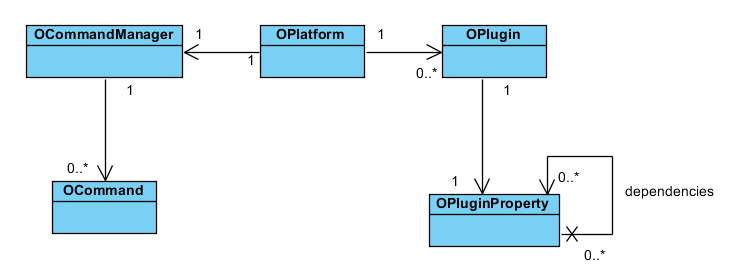
\includegraphics[width=10cm]{figures/class_diagram.png}

\subsection{Plugins}

\subsubsection{Création d'un nouveau plugin}

\subsection{Installation}

Tout d’abord, dans un terminal, tapez:
\begin{verbatim}
git clone https://github.com/masters-info-nantes/onyx.git
\end{verbatim}

Lorsque tous les fichiers sont téléchargés,vérifiez que le proxy de maven est correct en faisant:
\begin{verbatim}
nano /.m2/settings.xml
\end{verbatim}

Le fichier devrait ressembler à ça:
\begin{verbatim}
<settings>
    <proxies>
        <proxy>
            <id>example-proxy</id>
            <active>true</active>
            <protocol>http</protocol>
            <host>proxy.ensinfo.sciences.univ-nantes.prive</host>
            <port>3128</port>
        </proxy>
    </proxies>
</settings>
\end{verbatim}

Placez-vous dans le dossier où vous avez cloné le projet. 
Tapez la commande:
\begin{verbatim}
mvn clean install
\end{verbatim}

Pour lancer l'execution par défaut, tapez:
\begin{verbatim}
mvn exec:java-X
\end{verbatim}
